\documentclass[a4paper,10pt]{article}
\usepackage[utf8]{inputenc}

\usepackage{amssymb,amsmath,amsfonts,amsthm}
\usepackage{graphicx}
%opening
\title{A Mechanistic Model of the Auditory Cortex with Inhibitory Subtypes}
\author{Youngmin Park and Maria N. Geffen}
\usepackage{xcolor}
\usepackage{soul}
\usepackage{subfigure}
% \usepackage{hyperref}

\newcommand{\ymp}[1]{{\color{red}{#1}}}
\newcommand{\g}[1]{{\color{gray}{#1}}}
\newcommand{\orange}[1]{{\color{orange}{#1}}}

\newcommand{\crefrangeconjunction}{--}
\newcommand{\x}{\mathbf{x}}
\newcommand{\y}{\mathbf{y}}
% \newcommand{\v}{\mathbf{v}}
\newcommand{\w}{\mathbf{w}}
\newcommand{\uu}{\mathbf{u}}
\newcommand{\e}{\mathbf{e}}


\newcommand{\q}{\boldsymbol{\theta}}
\newcommand{\io}{\int_\Omega}
\newcommand{\ve}{\varepsilon}
\newcommand{\pa}{\partial}
\newcommand{\z}{\mathbf{z}}
\newcommand{\F}{\mathbf{F}}
\newcommand{\G}{\mathbf{G}}
\newcommand{\R}{\mathbb{R}}
\newcommand{\B}{\mathbf{B}}


\begin{document} 

\maketitle
\begin{abstract}
Abstract 
\end{abstract}
% \tableofcontents
 
\section{Introduction}

Complex auditory processing, such as habituating to harmless sounds, detecting sudden changes in the acoustic environment, and extracting important acoustic features from noise, are important to the survival of many animals. In the mammalian cortex, the auditory cortex (AC) is a key region for processing temporally complex sounds \cite{} and encodes responses to noise-gaps and noise-bursts \cite{}. In addition, the AC refines responses from earlier sensory pathways, sharpening direction selectivity \cite{} and frequency tuning curves \cite{}.

Various phenomena in AC are associated with complex temporal processing. For example, neurons are known to respond weakly to a frequent standard tone, but respond strongly to a rare deviant tone at a different frequency. This phenomenon is known as stimulus-specific adaptation (SSA) \cite{}. As another example of context-dependent responses, neurons respond substantially less to an acoustic stimulus when the preceding stimulus is similar in spectral content, a phenomenon known as forward suppression (FS) \cite{}. In addition to temporal adaptation, neurons adapt firing rates as a function of a spectro-temporally dynamic stimuli, a phenomenon known as gain adaptation \cite{}.

Tightly-coupled networks of excitatory and inhibitory neurons are responsible for generating these cortical responses. Indeed, current mechanistic models of AC use two idealized populations of excitatory and inhibitory neurons and successfully reproduce many cortical responses to temporally complex stimuli, including SSA \cite{mill2011neurocomputational,nelken2014stimulus,yarden2017stimulus} and FS \cite{loebel2007processing}. While such models are useful and informative, they do not account for the latest ground-breaking development in neuroscience: optogenetics.

Optogenetics allows researchers to manipulate the function of neural subpopulations classified by genetic markers \cite{markram2004interneurons,li2014differential} in real time \cite{deisseroth2006next}. In addition to pyramidal neurons -- excitatory neurons that make up over 80\% of cortical neurons \cite{} -- several recent studies implicate the two most common types of inhibitory neurons, parvalbumin- (PV) and somatostatin- (SOM) positive interneurons in processing complex sounds and identifying their specific roles in different auditory paradigms.

In stimulus-specific adaptation, inhibition of PVs reveal a constant inhibition throughout SSA, while inhibition of SOMs reveal an adapting inhibition \cite{natan2015complementary}. In forward suppression, PV (SOM) inactivation results in enhanced (reduced) forward suppression \cite{phillips2017cortical}. During tuning curve adaptation, PV inactivation results in increased neural activity at the sidebands with no change at the preferred frequency, while SOM activation results in increased neural activity at the preferred frequency following adaptation \cite{natan2017cortical}. Using white-noise burst stimuli, PVs identified using optogenetic techniques consistently respond earlier than other neurons \cite{keller2018gap} (fast PV responses appear to be a general property of PVs \cite{li2014feedforward}).

Optogenetics is of course not limited to complex stimuli. Optogenetic activation of PVs enhances functional connectivity in the thalamo-cortical circuit \cite{hamilton2013optogenetic}. PV or SOM activation each result in divisive and subtractive effects of tuning curves in similar ways \cite{phillips2016asymmetric,phillips2017diverse}.

In addition to function, the structure of PVs and SOMs are highly stereotyped: PVs synapse onto the perisomatic domain of neurons \cite{}, whereas SOMs synapse onto the distal apical dendrites of pyramidal neurons \cite{} -- a structural motif that repeats within AC \cite{} and other cortical regions \cite{}. These morphological differences are hypothesized to contribute to divisive and subtractive division of neural firing rates and tuning curves with conflicting reports \cite{}. Within this simple motif, there exist evidence for recurrent connections in SOMs \cite{} and PVs \cite{}. The role of these connections, and the specific circuits formed by these inhibitory neurons subtypes that support the reported phenomena remain unknown.

% To date, this knowledge of structure and function has not yet been sufficient to fully understand the cortical mechanisms underlying responses to auditory stimuli. How the cortex encodes auditory features remains unknown.


% However, the specific circuits formed by these inhibitory neurons subtypes that support the reported paradigms remain unknown.


% yet a mechanistic understanding of how neurons in AC respond to sounds under varying temporal contexts remains elusive.

% The existence of inhibitory subtypes have been known for some time, and identified using intrinsic membrane properties \cite{connors1990intrinsic} or genetic markers \cite{markram2004interneurons,li2014differential}. Due to the great success of modeling many cortical phenomena through the use of two-population inhibitory and excitatory models \cite{wilson1972excitatory,wilson1973mathematical}, modeling studies of inhibitory subtypes have appeared only very recently, spurred in large part to the development of optogenetics \cite{deisseroth2006next}.

% Modeling studies have explained and predicted the differential roles of interneurons in many cortical phenomena, including short term memory \cite{wang2004division}, cortical oscillations \cite{vierling2010computational}, visual surround suppression \cite{litwin2016inhibitory}, contextual visual processing \cite{lee2017computational}, auditory forward suppression \cite{phillips2017cortical}, stimulus-specific adaptation \cite{natan2015complementary}, and neural tuning \cite{litwin2016inhibitory,phillips2016asymmetric}.

% Despite this growing interest in extending mechanistic models to incorporate inhibitory subpopulations, most studies focus on the visual cortex with comparatively less studies in other cortical areas. In the auditory cortex, there are several experimentally-observed phenomena which have not yet been explained using mechanistic models.

% Inhibitory subtypes have been shown to exhibit differential effects on neural tuning curves during stimulus-specific adaptation \cite{natan2017cortical}, but the underlying mechanism has not been explored in earnest. In a separate result, activation of parvalbumin- (PV) positive interneurons result in enhanced functional connectivity in the thalamo-cortical circuit \cite{hamilton2013optogenetic}, but there is no known mechanistic cause of this increase. Further still, PVs consistently respond earlier than other neurons to white-noise bursts \cite{keller2018gap} and simple auditory stimuli \cite{li2014feedforward}, but the circuit-level cause of this fast response is not known.

Existing mechanistic models of the auditory cortex apply to the scale of the whole brain  \cite{jansen1995electroencephalogram,wang2013realistic}, or apply to auditory cortex but do not include inhibitory subtypes \cite{mill2011neurocomputational,loebel2007processing,yarden2017stimulus}. The few studies that include inhibitory subtypes are restricted to specific results. For example, models of forward suppression \cite{phillips2017cortical,phillips2017diverse} also account for differential interneuron modulation of tuning curves \cite{phillips2016asymmetric,seybold2015inhibitory}, but such models do not readily generalize to other temporally-dependent paradigms such as stimulus-specific adaptation, nor can they readily be adapted to predict other phenomena such as chances in functional connectivity. Likewise, an existing model of stimulus-specific adaptation with inhibitory subtypes \cite{natan2015complementary} does not generalize to tuning curve modulation during stimulus-specific adaptation, nor does it apply to forward suppression. The Ising model has been used to describe enhanced functional connectivity as a function of PV activation \cite{hamilton2013optogenetic}, but the mechanisms and the anatomical connections underlying this change is not known.

In the present study, we introduce a consistent mechanistic framework to aid in understanding the role of interneurons in processing dynamic auditory stimuli. Using this framework, we reproduce a range of results including SSA, FS, tuning curve adaptation, and changes in functional connectivity. Because all anatomical connections are known in the model, it naturally generates plausible causes of observed changes in the cortex. Given such a diverse set of phenomena, we naturally expect the model parameters to be very different from result-to-result, however, we find that only a single parameter set is sufficient.

More importantly, our model demonstrates synaptic depression only in the thalamo-cortical circuit is sufficient to reproduce temporally dynamic cortical responses of optogenetic studies, suggesting that synaptic plasticity of interneurons serve other functions, such as enhancing responses or improving robustness. While all our results use the lateral connections akin to those found in primary visual cortex (V1), namely lateral pyramidal-to-SOM synapses, we find that this lateral connection is necessary to reproduce the facilitating effects following SOM inactivation in forward suppression. This type of lateral connection is a proposed mechanism for surround suppression in V1 \cite{}, thus, this finding suggests that the mechanism of surround suppression in V1 exists in AC for a very different purpose.

%This novel framework adds to existing frameworks in other cortical regions \cite{litwin2016inhibitory}.

\section{Materials and Methods}

We consider three models in this paper. The first is an augmented version of the Wilson-Cowan model, consisting of a single iso-frequency unit of the auditory cortex consisting of one excitatory neural population and two inhibitory neural subpopulations. The second is a three-unit version of the augmented Wilson-Cowan. The third is a single-unit spiking model.

In the interest of maximizing the reproducibility and auditability of our results, all code used to generate the figures (including model simulations, numerical methods, and analysis tools) are available on GitHub at \texttt{insert github url here} under the MIT open source license. 

\subsection{Augmented Wilson-Cowan Model}
We draw much of our understanding of adaptation in the auditory cortex by using a model of a single iso-frequency unit.
\begin{equation}\label{eq:wc}
 \begin{split}
 \frac{d u(t)}{d t} &= -u(t) + f\left( K_{uu} u - K_{up} p - K_{es}s + q I(t) \right),\\
 \tau_p\frac{d p(t)}{d t} &= -p(t) + f\left( K_{pu} u - K_{pp}p - K_{ps}s + q I(t)\right),\\
 \tau_s\frac{d s(t)}{d t} &= -s(t) + f(K_{se}u - K_{sp}p - K_{ss}s),
 \end{split}
\end{equation}
where $u$ represents the normalized firing rate (scaled from 0 to 1) of the excitatory population, $p$ and $s$ represent the normalized firing rates of the inhibitory subpopulations PV and SOM, respectively. The function $f$ is either a sigmoid or a threshold linear function (such that $f(-\infty) = 0$ and $f(\infty)=1$). The sigmoidal firing rate is defined as
\begin{equation}\label{eq:sigmoid}
 f(x) = \frac{1}{1+\exp(-r x)},
\end{equation}
and the threshold linear function is defined as
\begin{equation}\label{eq:linear}
 f(x) = \left\{\begin{matrix}
         0 & \text{if} \quad x \leq 0\\
         r x & \text{if} \quad 0 < x \leq 1\\
         1 & \text{if} \quad x > 1
        \end{matrix}\right. .
\end{equation}
The parameter $r$ determines the gain of the firing-rate function. Thresholding may be added by writing $f(x-u_{th})$, where $u_{th}$ is a real number.

\begin{figure}
\centering
 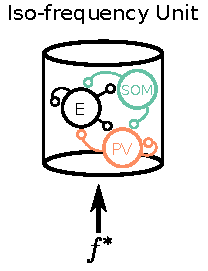
\includegraphics[]{col1.pdf}
 \caption{Iso-frequency unit model. Excitatory (Pyr) form recurrent connections with SOMs and PVs. Connectivity structure and synaptic weights as in Equation \eqref{eq:ssa_weights}. Iso-frequency auditory stimuli directly excite Pyr (E) neurons and PV (orange) interneurons.}\label{ref:col1}
\end{figure}


The input function $I(t)$ consists of blocks of inputs with stimulus interval $\delta$ms. When an auditory input arrives, the default temporal profile is taken to have an instantaneous rise with amplitude $q$ and exponential decay with time constant $\tau_q=10$ms. The input $I(t)$ is further modulated by a slow timecourse synaptic depression term $g$ satisfying
\begin{equation}\label{eq:thal}
 dg/dt = (g_0 - g)/\tau_{d_1} - I(t)/\tau_{d_2},
\end{equation}
where the time constants are $\tau_{d_1} = 1500$ms and $\tau_{d_2}=20$ms (chosen close to reported values \cite{natan2015complementary}). The variable $g$ effectively modulates the amplitude of auditory inputs to A1 over long times.

In Figure \ref{fig:wc_space}, each unit shows the connectivity pattern based on existing studies on AC \cite{pfeffer2013inhibition}. The connectivity is equivalently represented by the matrix,
\begin{equation}\label{eq:ssa_weights}
 W = \left(\begin{matrix}
      1.1 & 2 & 1\\
      1   & 2 & 2\\
      6   & 0 & 0
     \end{matrix}\right),
\end{equation}
All synapses in the rate model are constant (as in \cite{mill2011neurocomputational}) except for the depressing feedforward thalamic inputs \cite{lee2008synaptic}.

Standard responses of the augmented Wilson-Cowan are shown in Figure \ref{fig:awc}. The top panel displays the timecourse of all neural populations including Pyr (black), SOM (green), and PV (dashed orange). These responses represent dimensionless population activity, where 0 represents a baseline or below-threshold firing rate, and 1 represents the maximum possible firing rate. The gray line represents the timecourse of the depressing thalamic input, which is also dimensionless in this model. The thalamic input profile is 
shown in the bottom panel (blue).

\begin{figure}[ht!]
\centering
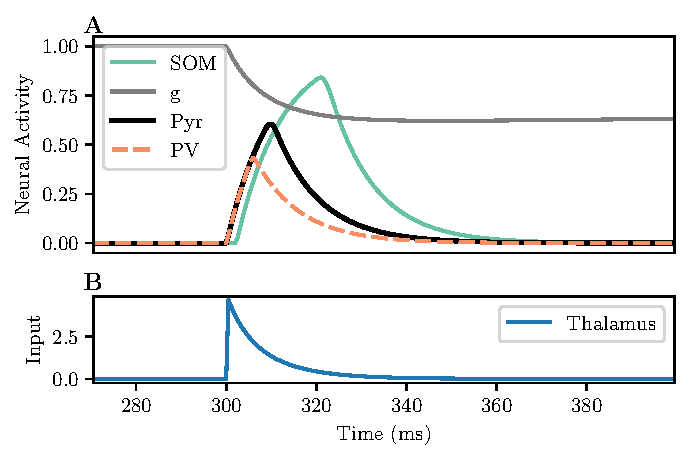
\includegraphics[width=.75\textwidth]{rate_responses.pdf}
 \caption{Input and response profiles of the single-unit model. Gray: The thalamic depression variable $g$. Black: Pyramidal neuron activity. Dashed orange: PV interneuron activity. Green: SOM interneuron activity. Blue, bottom panel: Thalamic inputs. The tone onset occurs at 300ms. While the tone duration lasts for 100ms, fast timescale thalamic adaptation quickly depresses the auditory input. $q=5$.}\label{fig:awc}
\end{figure}


Because both PVs and Pyrs receive direct thalamic inputs, their activation coincide, but PVs peak earlier, in agreement with existing studies \cite{keller2018gap}. Because synapses between excitatory and inhibitory neurons are static, this feature is a result of the connectivity pattern and not due to synaptic effects. The delay in SOM activation is caused by a lack of direct thalamic inputs. SOMs instead receive excitatory input from the Pyr population with a high threshold, making SOM activation dependent on Pyr activity, which occurs on a slower timescale than thalamic inputs.

An important feature of this model is the early, fast temporal activation of PVs and the late, broad temporal activation of SOMs. While the total inhibition is active both before and well after the peak activation of Pyrs, the differential inhibition of PVs and SOMs result in nontrivial changes to Pyr activity. In section \ref{sec:adaptation}, we demonstrate how simple changes in PV and SOM activity alter Pyr activity in ways that mimic optogenetic results in SSA. We then extend this model to include a tonotopy (Section \ref{sec:awc3}), and show that the model coincides strikingly well with many different optogenetic results.

\subsection{Three-unit Rate Model}\label{sec:awc3}
We take the single-unit rate model and arrange copies into three units with lateral cortical and thalamic connections (Figure \ref{fig:wc_space}). This arrangement endows our model with a gross tonotopy, which we  use to explore spectrally complex auditory inputs in addition to temporally dynamic sounds.

\begin{figure}[ht!]
\centering
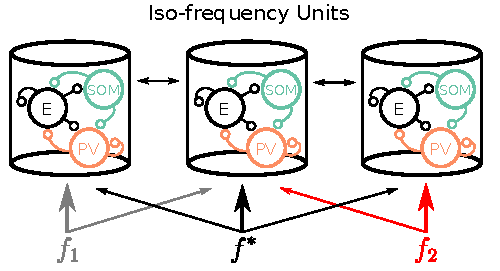
\includegraphics[width=.75\textwidth]{col3.pdf}
\caption{A visual representation of the augmented Wilson-Cowan model with three units.}\label{fig:wc_space}
\end{figure}

The first, or leftmost unit, satisfies
\begin{align*}
 u_1' &= u_1 + f( w_{uu} u_1 - w_{up}p_1 - w_{us}s_1 + qI_1(t) + w_{uu}^* u_2),\\
 \tau_p p_1' &= p_1 + f( w_{pu} u_1 - w_{pp}p_1 - w_{ps}s_1 + qI_1(t) + w_{pu}^* u_2),\\
 \tau_s s_1' &= s_1 + f( w_{su} u_1 - w_{sp}p_1 - w_{ss}s_1 + w_{su}^* u_2),
\end{align*}
where $I_1 = i_1(t) +i_2(t)\alpha$. The second, or center unit, satisfies
\begin{align*}
 u_2' &= u_2 + f( w_{uu} u_2 - w_{up}p_2 - w_{us}s_2 + qI_2(t) + w_{uu}^* (u_1+u_3)/2),\\
 \tau_p p_2' &= p_2 + f( w_{pu} u_2 - w_{pp}p_2 - w_{ps}s_2 + qI_2(t) + w_{pu}^* (u_1+u_3)/2),\\
 \tau_s s_2' &= s_2 + f( w_{su} u_2 - w_{sp}p_2 - w_{ss}s_2 + w_{su}^* u_2),
\end{align*}
where $I_2(t) = (i_1(t)+i_3(t))\alpha +i_2(t)$. Finally, the third, or right unit, satisfies
\begin{align*}
u_3' &= u_3 + f( w_{uu} u_3 - w_{up}p_3 - w_{us}s_3 + qI_3(t) + w_{uu}^* u_2),\\
 \tau_p p_3' &= p_3 + f( w_{pu} u_3 - w_{pp}p_3 - w_{ps}s_3 + qI_3(t) + w_{pu}^* u_2),\\
 \tau_s s_3' &= s_3 + f( w_{su} u_3 - w_{sp}p_3 - w_{ss}s_3 + w_{su}^* u_2), 
\end{align*}
where $I_3 = i_2(t) +i_3(t)\alpha$. The parameters $\tau_p,\tau_s$ are membrane time constants. The function $f$ is sigmoid (Equation \eqref{eq:sigmoid}) or threshold linear (Equation \eqref{eq:linear}). The functions $I_k(t)$ are time-dependent inputs with the strongest preference for unit $k$. The parameter $q$ controls the strength of all inputs. Each input $i_j(t)$ is modulated by its own thalamic variable $g_i$, where each $g_i$ satisfies Equation \eqref{eq:thal} independently.

\begin{figure}[ht!]
\centering
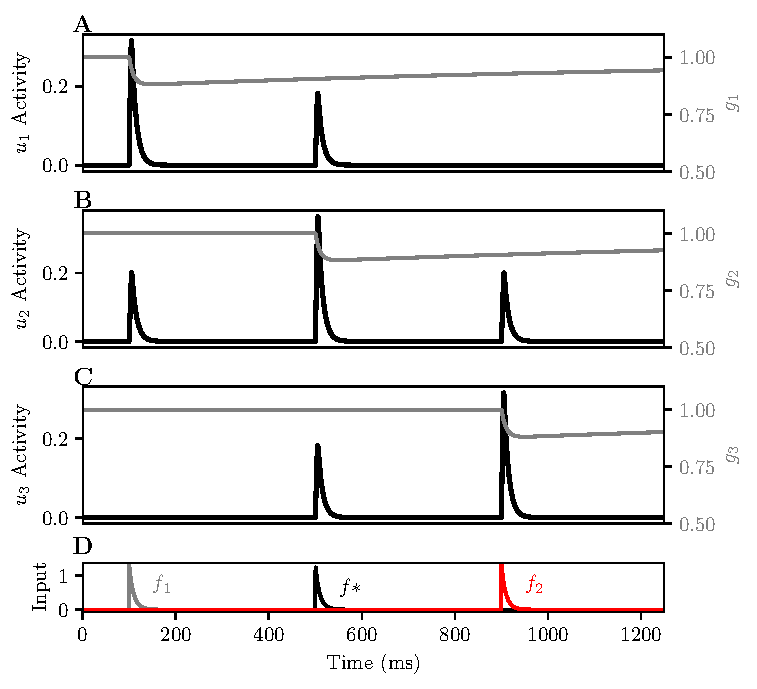
\includegraphics[width=.75\textwidth]{rate_responses3.pdf}
 \caption{Input and response profiles of the three-unit model. Auditory inputs are applied at each frequency in sequence. The traces of the auditory inputs are shown in panel D: $f_1$ (gray), $f^*$ (black), and $f_2$ (red). The black traces in panels A--C show the excitatory cortical response of the first ($u_1$), second ($u_2$), and third ($u_3$) units, respectively. $q=1.3$.}\label{fig:3unit}
\end{figure}


In Figure \ref{fig:3unit}, we apply three successive auditory stimuli in order of the frequencies $f_1$, $f^*$, and $f_2$, thus stimulating the left, center, and right units, respectively. The top three panels show the excitatory response in black, as well as the thalamic depression $g_i$ in gray. The center unit ($u_2$) responds equally well to both $f_1$ and $f_2$, which is a necessary response for SSA paradigms. For simplicity, activation of an adjacent unit does not affect the thalamic variable, i.e., $g_1$ is unaffected by $u_2$ activity, $g_2$ is unaffected by $u_1$ and $u_2$ activity, and $g_3$ is unaffected by $u_2$ activity. We assume that the frequency difference between $f_1$ and $f_2$ is great enough that auditory inputs at $f_1$ ($f_2$) do not affect units responsive to $f_2$ ($f_1$).


% At the extremes of the tonotopy are two units that satisfy the system
% \begin{equation}\label{eq:wc_space2}
%  \begin{split}
%  \frac{d u_1(t)}{d t} &= -u_1 + f\left(w_{uu} u_1 - w_{up}p_1 - w_{us}s_1 \right),\\
%  \tau_p\frac{d p_i(t)}{d t} &= -p_i(t) + f\left(\sum_{k=i-1}^{i+1} \left[\beta_{k-i} u_i + q_{k-i} I_k(t) \right] - K_{pp}p_i - K_{ps}s_i \right),\\
%  \tau_s\frac{d s_i(t)}{d t} &= -s_i(t) + f(K_{se}u_i - K_{sp}p_i - K_{ss}s_i),
%  \end{split}
% \end{equation}



% When using Equation \eqref{eq:wc_space} to reproduce cortical phenomena, we 

% Although VIP-expressing interneurons are almost as common as PVs and SOMs \cite{pfeffer2013inhibition} with well-established properties \cite{mesik2015functional,ji2015thalamocortical}, we do not include VIPs in this model to reduce the degrees of freedom.



\subsection{Spiking Neuron Dynamics}

The second model type we consider is a spiking model. All inhibitory neurons consist of a single somatic compartment, while the excitatory neurons are two-compartment, ``ball-and-stick'' models. For each excitatory and inhibitory neuron, the somatic (ball) compartment is an adaptive exponential integrate-and-fire model \cite{brette2005adaptive,litwin2016inhibitory}:
\begin{equation*}
 \begin{split}
  C_m \frac{dV^A_i}{dt} &= I_i^A -g_L (V^A_i-E_L) - w^A_i + g_L^A \Delta_T^A e^{(V^A_i-V_T^A)/\Delta_T^A} \end{split}
\end{equation*}
where the transmembrane currents are $I_i^A = I_{\text{Syn},i}^A + I_i^A(t)$
\begin{align*}
 I_{\text{Syn},i}^A &= -\sum_{B}g_{AB,i}(t)(V_i^A(t)-E_\text{Syn}^B),\\
 I^A_i(t) &= I_{\text{baseline},i}^A + I_{\text{external},i}^A(t),
\end{align*}
and we perturb each somatic compartment with a white noise process (zero mean and a standard deviation of $20$mV) to simulate intrinsic membrane fluctuations. For an excitatory neuron ($A=e$), the transmembrane currents are $I_i^A = I_{\text{Syn},i}^A + I_i^A(t)$, where
\begin{equation*}
 I_\text{Dend} = -g_{sd}(V_E-V_D)/(1-\kappa),
\end{equation*}
and the sum $\sum_B$ iterates over the inhibitory interneurons, $B\in \{p,s\}$.
The parameters $E_E=0$mV and $E_I=-67$mV represent excitatory and inhibitory reversal potentials, respectively. The variable $w$ represents spike-frequency adaptation and obeys
\begin{equation*}
 \tau_w\frac{dw_E}{dt} = a\left(V_E - E_L\right) - w_E(t).
\end{equation*}
Following a presynaptic spike from neuron $i$, the postsynaptic effect on neuron $j$ appears as an instantaneous spike in the postsynaptic conductance $g_{ij} \rightarrow g_{ij} + g_{ij,\text{max}}/n_\text{X}$, where $g_{ij,\text{max}}$ is given by Equation \eqref{eq:cond}, and X stands for the presynaptic neuron type (Pyr, PV, or SOM).

\begin{figure}[ht!]
\centering
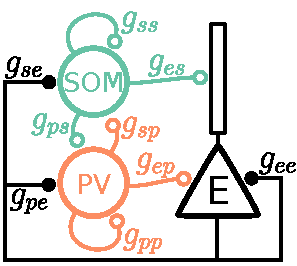
\includegraphics[width=.3\textwidth]{spiking_conn2.pdf}
\caption{A visual representation of the spiking network motif. The variables $g_{ij}$ place the location of each conductance variable in the microcircuit. The excitatory pyramidal neuron (black) consists of two compartments, the soma and apical dendrite, while PV (orange) and SOM (teal) interneurons consist of a single compartment.}\label{fig:spike}
\end{figure}

\begin{equation}\label{eq:cond}
 G_{\text{max}} = \left(\begin{matrix}
  g_{ee,\text{max}} & g_{ep,\text{max}}  & g_{es,,\text{max}} \\
  g_{pe,\text{max}}  & g_{pp,\text{max}}  & g_{ps,\text{max}} \\
  g_{se,\text{max}} & g_{sp,\text{max}}  & g_{ss,\text{max}} 
 \end{matrix}\right)= \left(\begin{matrix}
  100  & 40  & 10 \\
  2  & 20  & 12.2 \\
  200  & 0  & 0 
 \end{matrix}\right)\text{nS}.
\end{equation}

In the absence of presynaptic spikes, the conductances $g_{ij}$ decay exponentially to zero:
\begin{equation*}
 \frac{dg_{ij}}{dt} = -g_{ij}/\tau_{ij},
\end{equation*}
where $\tau_{ij} = 1$ms for all neurons except for the time constants from pyramidal to PVs, $\tau_{pe} = 25$ms, and pyramidal to SOMs, $\tau_{se} = 15$ms.


\begin{figure}[ht!]
 \centering
 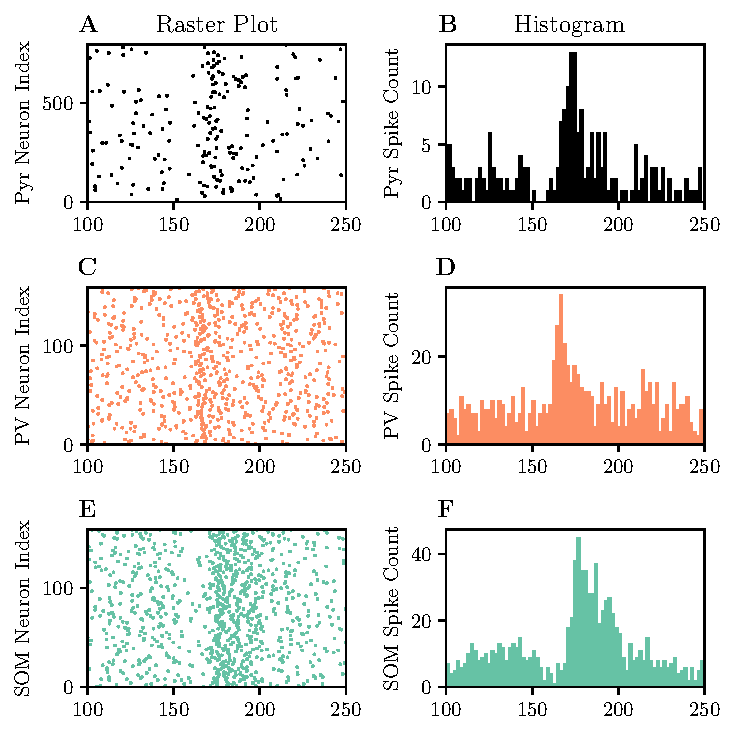
\includegraphics[width=.75\textwidth]{spike_responses.pdf}
 \caption{Raster plot and spike count for each neural population in response to one auditory stimulus. A: Raster plot of the excitatory population, with corresponding spike-count histogram (B). C: Raster plot of the PV interneuron population, with corresponding spike-count histogram (D). E: Raster plot of the SOM interneuron population, with corresponding spike-count histogram (F).}
\end{figure}


The dynamics of the dendritic (stick) compartment obey
\begin{equation*}
 C_m \frac{dV_D}{dt} =  -g_L(V_D-E_L) - g_{sd}(V_D-V_E)/\kappa-g_{es}(t)(V_D-E_I).
\end{equation*}

The parameter $\kappa=0.3$ is the ratio of somatic to total surface area \cite{}.


\begin{table}
\caption{Parameter values of spiking neurons.}\label{tab:spike}
\centering
\begin{tabular}{ c|c|c|c|c } 
 %\hline
       & Pyr & Dend & PV & SOM\\ 
 \hline
 $C_m$ (pF) & 180  & 180  & 80  & 80 \\
 $I_L$ (mV) & -60  & -60  & -60 & -60 \\ 
 $g_L$ (nS) & 6.25 & 6.25 & 5   & 5 \\
 $\Delta_T$ (mV) & 1 & - & 0.25 & 1\\
 $V_T$ (mV) & -40 & - & -40 & -45\\
 $V_\text{reset}$ (mV) & -60 & - & -60 & -60\\
 $g_{sd}$ (nS) & 18.75 & 18.75 & 0 & 0\\
 $I_\text{baseline}$ (nA) & 0.35 & - & 0.05 & 0.025
%  \hline
\end{tabular}
\end{table}



\subsection{Three-unit Spiking Model}

In order to introduce tonotopy into the spiking model, we introduce a gross tonotopy by arranging the single unit spiking model into three distinct units with lateral excitatory connections. The connectivity structure is identical to the rate model (Figure \ref{fig:3unit}).



\section{Results}

Adaptation, the reduced neural response to repeated stimuli, is a key feature of the auditory cortex. Adaptation is a necessary part of normal function and survival, considering that sources of danger such as predators or natural disasters can cause sudden changes in the acoustic environment.

In this section, we demonstrate that the augmented Wilson-Cowan model (Equation \eqref{eq:wc_space}) is sufficient to reproduce the latest optogenetic results in cortical adaptation.

\subsection{Adaptation}\label{sec:adaptation}

We hypothesize that a single iso-frequency unit contains the necessary mechanisms behind stimulus-specific adaptation and forward suppression. As such, we first seek to reproduce the results of Natan et al. 2015, in particular the constant disinhibition due to PV inactivation, and the increasing disinhibition due to SOM inactivation. However, instead of using an SSA paradigm, we started with a simple sequence of five single tones, and treat the first tone as a surrogate for the deviant tone, and each tone thereafter as post-deviant tones. The simplicity of this starting point allows us to create and understand a plausible circuit mechanism for SSA and forward suppression.

In Figure \ref{fig:adaptation}, we show that a single-unit model with constant synapses and depressing thalamic inputs are sufficient to reproduce SSA-like results. The two key features of the mechanism behind this result is the temporal structure of the responses and the thresholds. In the control case, for each tone, PVs respond first, while SOMs respond later and for longer. Due to thresholding of the SOM response, the SOM response is effectively delayed by several milliseconds, in possible agreement with existing results \cite{natan2015complementary}.

With PV inactivation, the constant disinhibition of the excitatory activity is due to the fact that only PVs are active at tone onset. There is no SOM activity that can compensate for the lack of PVs, resulting in a greater response across all deviant and post-deviant tones.

With SOM inactivation, at the deviant tone, PV activity compensates for SOM inactivation, thus there is no net change in the response of the excitatory population. In post-deviant tones, and in particular following adaptation, PV activity is relatively weak and does not compensate for the lack of SOM activity. Thus, excitatory neurons become disinhibited, showing increased activity.


\begin{figure}
\caption{Adaptation figure.}\label{fig:adaptation}
\end{figure}


\subsection{Stimulus-Specific Adaptation}\label{sec:ssa}

% \begin{figure}[ht!]
% \centering
% \includegraphics[width=.3\textwidth]{ssa_weights.pdf}
% \caption{Synaptic weights for stimulus-specific adaptation and forward suppression \cite{pfeffer2013inhibition}. The spatial arrangement remains as in Figure \ref{fig:awc}.}\label{fig:ssa_weights}
% \end{figure}


Auditory stimulus-specific adaptation (SSA) manifests as a decrease in cortical response to a repeating auditory stimulus (standard) that does not generalize to another rarely-occuring stimulus (deviant) \cite{yarden2017stimulus}. SSA is a robust and well-documented cortical phenomenon in various animal models including cats \cite{ulanovsky2003processing}, rats \cite{von2009correlating}, and mice \cite{natan2015complementary,natan2017cortical}.

There exist many comprehensive mechanistic models of SSA. Mill et al. (2011), use multple configurations of spiking neuron populations, consisting of inhibitory and excitatory neurons, to reproduce cortical responses to oddball sequences used in SSA experiments \cite{mill2011neurocomputational}. Mill et al. (2012) use a two-layer rate model with synaptic depression to quantify the relationship between the cortical response and the parameters in SSA experiments, such as stimulus frequency differences, probability of deviation, and tone presentation rate \cite{mill2012characterising}. Yarden et al. (2017) use a multi-unit rate model arranged on a coarse tonotopy consisting of inhibitory and excitatory populations \cite{yarden2017stimulus}. Each study advances our understanding of the basic mechanisms underlying SSA, however, they do not account for multiple inhibitory subtypes, and their differential roles as discovered in recent optogenetic experiments. 



\begin{figure}[ht!]
 \centering
 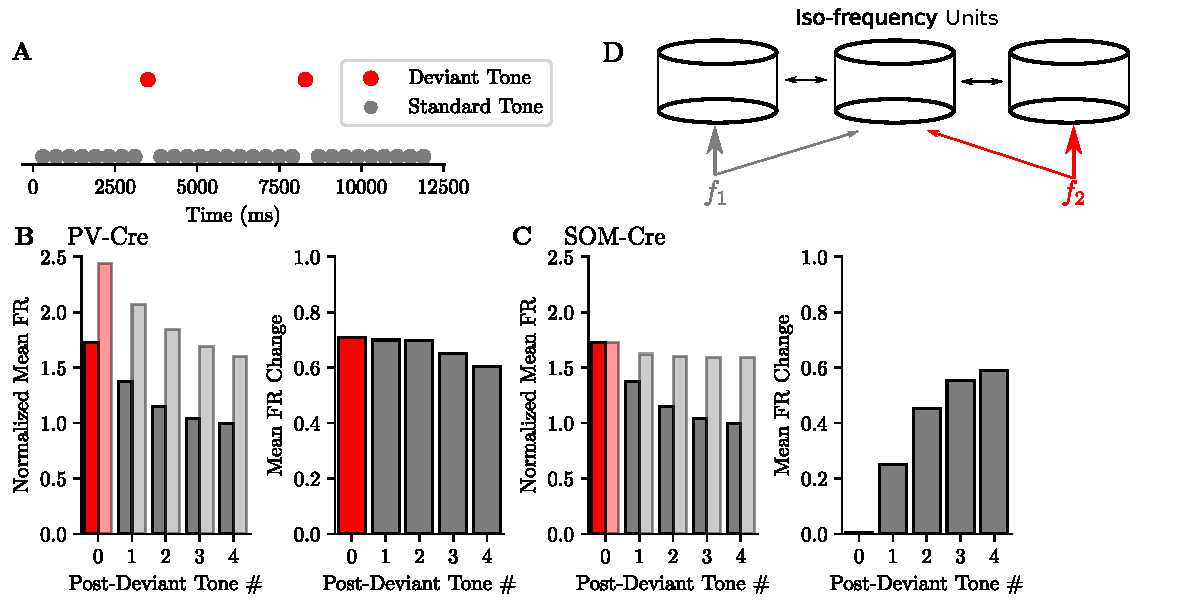
\includegraphics[width=\textwidth]{ssa.pdf}
 \caption{Summary of stimulus-specific adaptation in a two-tone paradigm. A: The timing of standard and deviant tones used in this model. Standard tones (gray) appear with 95\% probability, while deviant tones (red) appear with 5\% probability. B: PV inactivation results in a near-uniform increase in firing rates (FR) through all post-deviant tones. C: SOM inactivation reveals a gradually increasing inhibitory effect. Both panels B and C qualitatively reproduce experimental results \cite{natan2015complementary}.}
\end{figure}


\subsection{Forward Suppression}

In forward suppression, neural responses to a sound are often abolished when preceded by a spectrally similar sound and more weakly suppressed when preceded by a spectrally dissimilar sound \cite{phillips2017cortical,phillips2017diverse}.

In Figure \ref{fig:fs}, we reproduce the differential roles of SOM and PV interneurons on forward suppression, in particular Figure 3A and 3C in Phillips et al 2017 \cite{phillips2017cortical}. Strikingly, we use the same connectivity parameters as in stimulus-specific adaptation (Section \ref{sec:ssa}), with only slight changes to the input strength and input timing. In particular, the input strength to reproduce forward suppression is weaker than that used to generate stimulus-specific adaptation. These differences agree with the experimental paradigm, where the auditory stimulus used in SSA was 65dB sound pressure level (SPL), whereas the auditory stimulus in forward suppression was at least 45dB.

\begin{figure}[ht!]
 \centering
 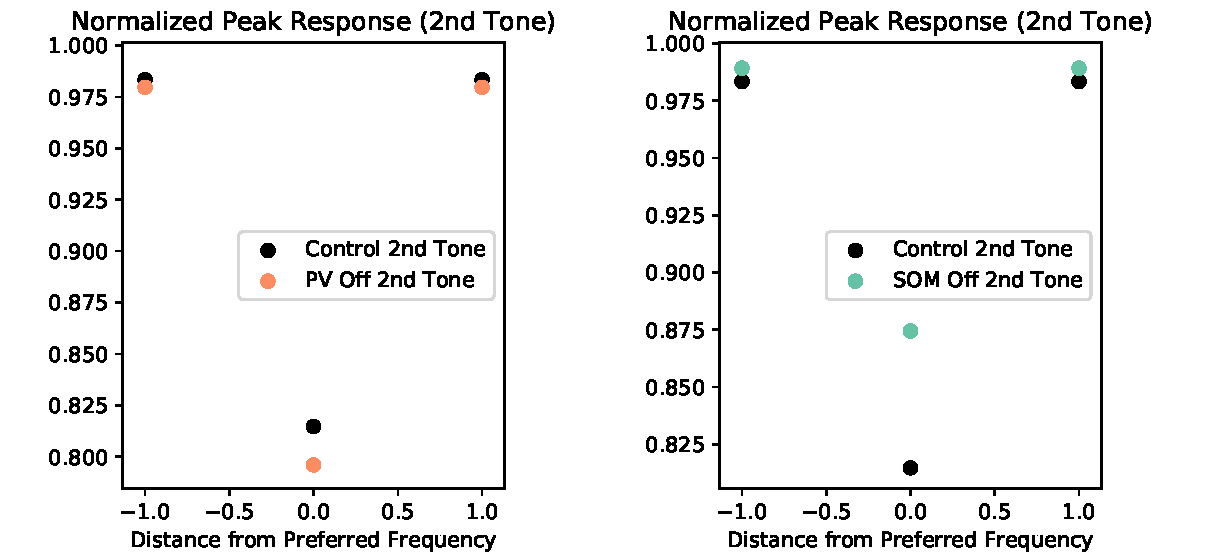
\includegraphics[width=\textwidth]{fs.pdf}
 \caption{Summary of forward suppression. A: Disinhibition of PV (orange) results in greater probe alone (PA) responses compared to the control (black). B: Normalizing by the PA tone shows that PV inhibition enhances forward suppression, in agreement with experiments. C: Disinhibition of SOM (teal) results in greater PA responses compared to the control (black). D: Normalizing by the PA tone shows that SOM inhibition results in reduced forward suppression and enhanced sideband facilitation, in agreement with experiments.}\label{fig:fs}
\end{figure}


\subsection{Tuning Curve Adaptation}

Researchers have long established the properties of neural adaptation to repeated tone-pips. To better understand neural responses during adaptation, recent work has turned to neural adaptation over multiple frequencies, establishing the properties of entire tuning curves during adaptation, and the differential roles of interneurons in modulating tuning curves over the course of adaptation. At the preferred frequency, inhibition of PVs result in no change before and after adaptation, while inhibition of SOMs result no change before adaptation and significant disinhibition after adaptation. At the sidebands, both PV and SOM inhibition result in disinhibition before and after adaptation.

\subsection{Enhanced Functional Connectivity}



%See \cite{kato2017network} for inhibition of recurrent connections.
% 
% \subsection{Mechanisms of Subtractive and Divisive Inhibition}
% 
% There exist many established mechanisms of subtractive and divisive inhibition in the modeling and experimental literature and exist at several scales, from the single-neuron spiking-level \cite{abbott_synaptic_1997,chance2002gain}, to the other extreme using a coarse-grained continuum-limit of neurons \cite{litwin2016inhibitory}.
% 
% The literature is futher complicated by ongoing debates on the role of interneurons on divisive and subtractive inhibition. At the spiking level, PVs serve a plausible mechanism for divisive inhibition because PV axons project onto the perisomatic synapses, directly affecting the membrane conductance \cite{chance2000divisive}. In contrast, SOMs serve a plausible mechanism for subtractive inhibition due to the distal synaptic connection \cite{yavorska2016somatostatin}, which only affects the input current to the perisomatic domain \cite{sturgill2015somatostatin}.
% 
% Despite the large body of evidence supporting differential effects at the spiking-level, these sharp distinctions blur at the population level. Both PV and SOM activation reveal equal divisive and subtractive effects on neural tuning curves \cite{seybold2015inhibitory}. or inactivation reveal divisive or subtractive effects \cite{}. There exist coarse-grain mechanistic models to explain this effect \cite{}, but these models do not generalize readily for use in modeling other phenomena.
% 

% 
% \subsection{Inhibitory Stabilized Networks in the Auditory Cortex}
% 
% % Rapid Rebalancing of Excitation and Inhibition
% 
% Many experimental and theoretical studies establish that the suppression of inhibitory neurons may result in the increase in both inhibitory and excitatory activity \cite{tsodyks1997paradoxical}. Such phenomena result from inhibitory stabilized networks (ISNs). ISNs have been used to explain phenomena in the primary visual cortex (V1) including selective amplificiation of neural activity \cite{murphy2009balanced}, surround suppression \cite{ozeki2009inhibitory}, and in the rat hippocampus \cite{tsodyks1997paradoxical}.
% 
% In this section, we reproduce two recent studies that present evidence for ISNs in the auditory cortex. In the first study, inhibitory post-synaptic currents (IPSCs) and excitatory post-synaptic currents (EPSCs) increase upon optogenetic inactivation of SOMs, with identical increases observed upon inactivation of PVs \cite{kato2017network}. The authors note that a transient decrease in IPSC, which occurs over the course of tens of milliseconds, precedes the IPSC increase, which occurs over the course of hundres of milliseconds.
% 
% % In contrast to \cite{litwin2016inhibitory}, where they characterize the ISN state by changes in the net input currents, we characterize the ISN state by the firing rates, in agreement with experimental studies \cite{moore2018rapid}.
% 
% We summarize our result in Figure \ref{fig:isn}. In order for an ISN to exist in the pyramidal and PV subpopulations, we require that SOMs either have a weak influence on PVs, or that PVs strongly suppress SOMs.
% 
% 
% \begin{figure}[ht!]
%  \centering
%  \includegraphics[width=\textwidth]{wehr_2018.pdf}
%  \caption{Neural responses in a non-inhibitory stabilized network (non-ISN) versus an ISN. A: Non-ISN state with no PV inhibition. B: Non-ISN with weak PV inhibition results in decreased PV response and increased pyramidal response. C: ISN state with no PV inhibition. D: ISN state with PV inhibition results in increased PV and pyramidal responses in agreement with experiments. In all cases we observe a small increase in SOM responses following PV inhibition.}\label{fig:isn}
% \end{figure}
% 


\appendix

\section{Beyond Three Units}

In the most general case of $N$ units, the $N-2$ center units satisfy the system
\begin{equation}\label{eq:wc_space}
 \begin{split}
 \frac{d u_i(t)}{d t} &= -u_i(t) + f\left(\sum_{k=i-1}^{i+1} \left[\alpha_{k-i} u_k +  q_{k-i} I_k(t) \right]- K_{ep}p_i - K_{es}s_i \right),\\
 \tau_p\frac{d p_i(t)}{d t} &= -p_i(t) + f\left(\sum_{k=i-1}^{i+1} \left[\beta_{k-i} u_i + q_{k-i} I_k(t) \right] - K_{pp}p_i - K_{ps}s_i \right),\\
 \tau_s\frac{d s_i(t)}{d t} &= -s_i(t) + f(K_{se}u_i - K_{sp}p_i - K_{ss}s_i),
 \end{split}
\end{equation}
were $i=2,\ldots,N-1$, $\delta_k$ is the Kronecker delta, $\alpha_k = \delta_k K_{ee} + (1-\delta_k)w_{ee}^*/2$, $q_k = \delta_k q_1  + (1-\delta_k)q_2$


\bibliographystyle{plain}
\bibliography{../audio,../computation,../cortex,../bio,../machines,../math}


\end{document}
